\chapter{Quantitative Study}

\section{Participants General Information}
\begin{figure}[H]
\centering
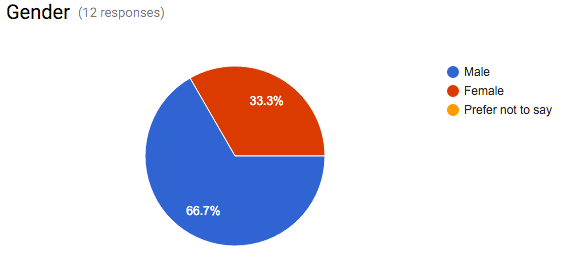
\includegraphics[width=13cm]{genderpie}
\caption{Pie Chart of Participants Gender \label{genderpie}}
\end{figure}



\begin{table}[H]
\centering
\caption{Participants Ages \label{agetable}}
\begin{tabular}{llllll}
\hline
  & Count & Min & Max & Mean & Std. Dev \\ \hline
Age  & 12 & 18 & 25 & 21.33 & 2.57  \\ \hline
\end{tabular}
\end{table}


\section{Previous Experience}

\begin{figure}[H]
\centering
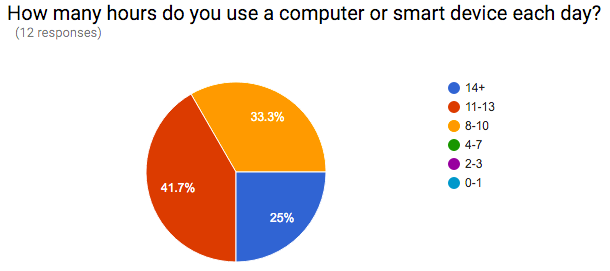
\includegraphics[width=13cm]{deviceusage}
\caption{Pie Chart of Participants Device Usage \label{deviceusage}}
\end{figure}

\begin{figure}[H]
\centering
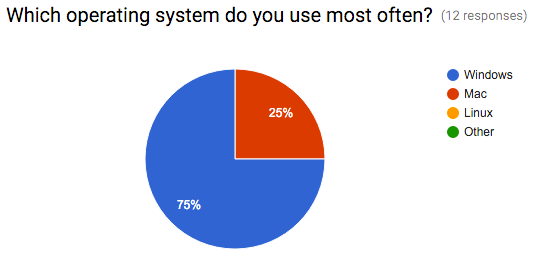
\includegraphics[width=13cm]{osusage}
\caption{Pie Chart of Participants Operating System Usage \label{osusage}}
\end{figure}

\begin{figure}[H]
\centering
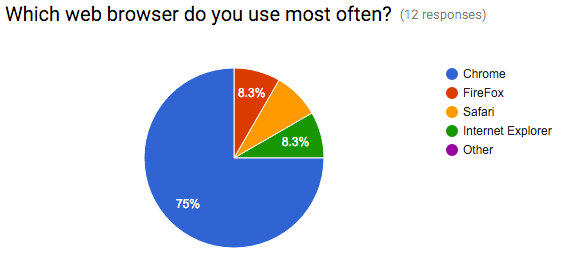
\includegraphics[width=13cm]{webbrowserusage}
\caption{Pie Chart of Participants Browser Usage \label{webbrowserusage}}
\end{figure}

\section{Code Reuse}

\begin{figure}[H]
\centering
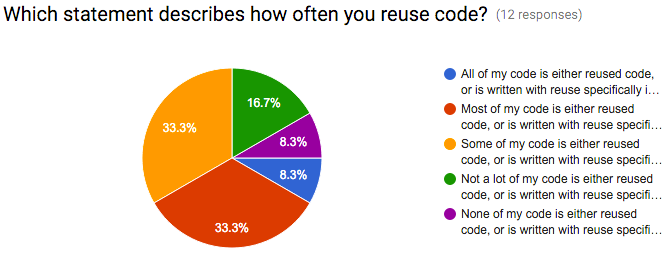
\includegraphics[width=13cm]{codereuseoften}
\caption{Pie Chart of Participants Current Code Reuse \label{codereuseoften}}
\end{figure}

\begin{figure}[H]
\centering
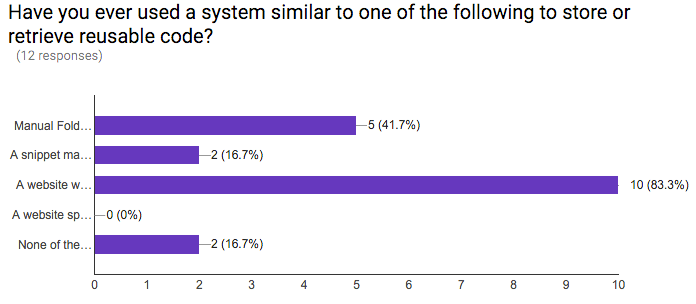
\includegraphics[width=13cm]{systemusebarchart}
\caption{Bar Chart of Participants Experience with Existing Systems \label{systemusebarchart}}
\end{figure}

\section{Initial Questionnaire} \label{appendixquestionnaires}

\begin{figure}[H]
  \centering
  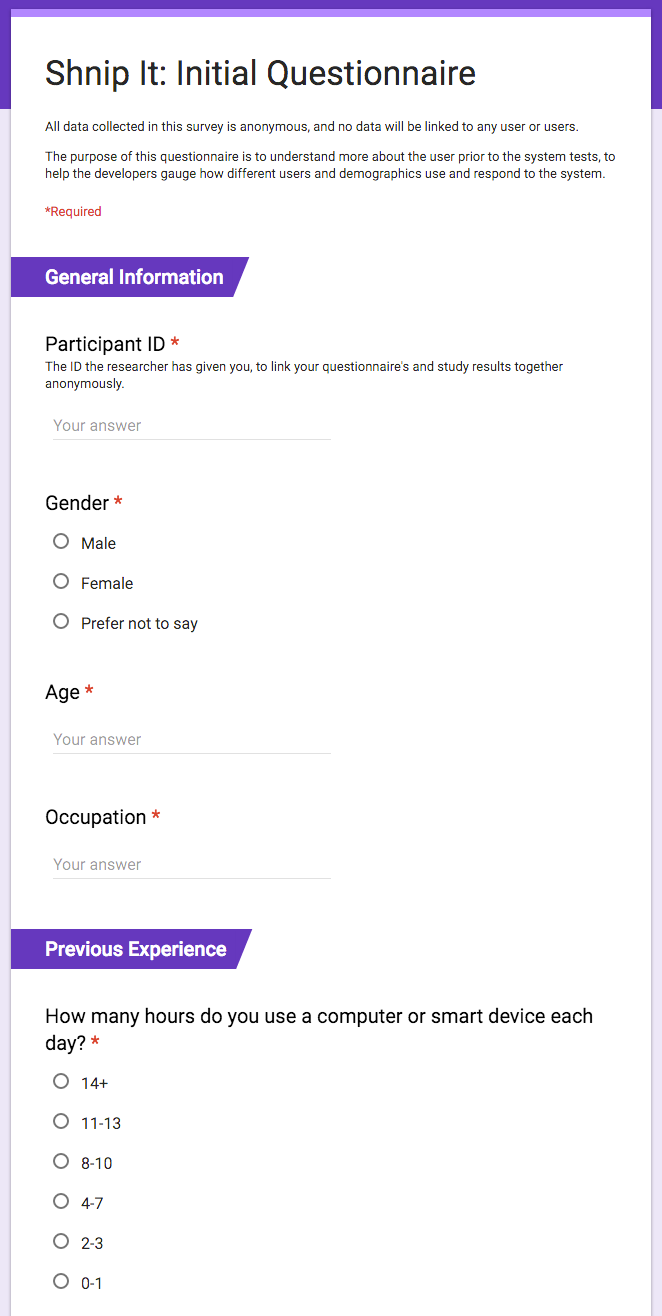
\includegraphics[width=10cm]{firstquest1}
  \caption{Initial Questionnaire \label{initialquestionnaire}}
\end{figure}

\begin{figure}[H]
  \ContinuedFloat
  \captionsetup{list=off,format=cont}
  \centering
  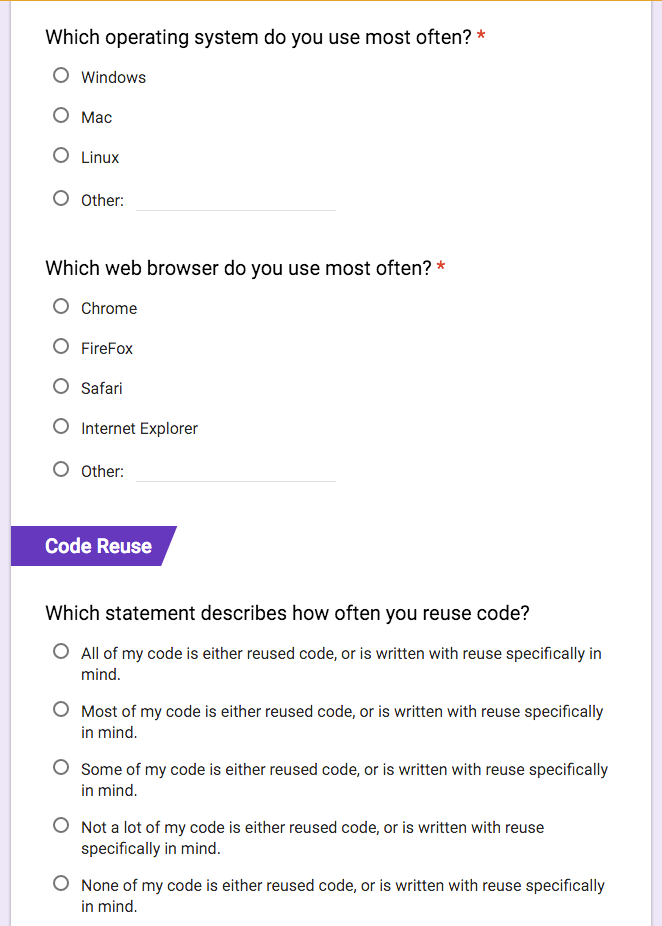
\includegraphics[width=10cm]{firstquest2}
  \caption{First figure continued}
\end{figure}

\begin{figure}[H]
  \ContinuedFloat
  \captionsetup{list=off,format=cont}
  \centering
  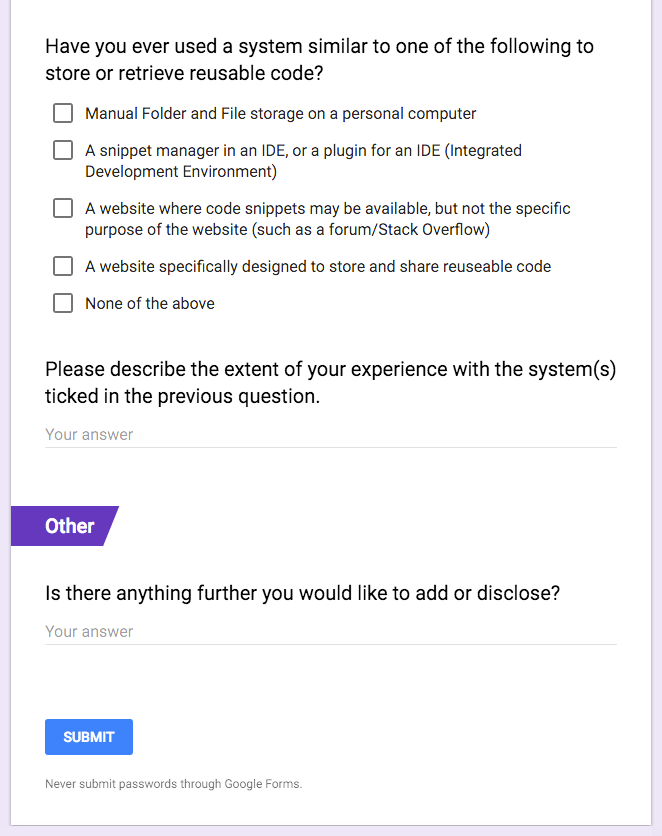
\includegraphics[width=10cm]{firstquest3}
  \caption{First figure continued}
\end{figure}

\section{Permission Slips} \label{appendixpermission}
\begin{figure}[H]
  \centering
  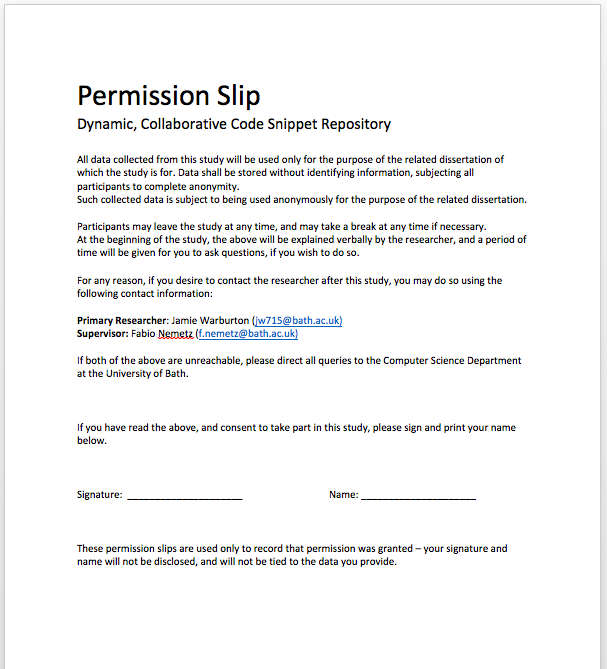
\includegraphics[width=13cm]{permissionslip}
  \caption{Study Permission Slip \label{permissionslip}}
\end{figure}



